\documentclass{article}
\usepackage{graphicx} % Required for inserting images
\usepackage{tikz}
\usetikzlibrary{positioning,arrows}
\usetikzlibrary{arrows.meta}
\usepackage{multirow}
\title{Portfolio report}
\usepackage{pgf-pie}  
\usepackage{subcaption}
\usetikzlibrary {datavisualization} 
\usepackage{pgfplots}
\date{\today}
\begin{document}
\maketitle
\tableofcontents      
\section*{Returns and overall performance}
\subsection*{Biggest positive and negative returns}
\begin{tikzpicture}

    \node[circle] at (0,1) {AAPL};
    
   \draw[-{Triangle[width=18pt,length=8pt]}, line width=8pt, color=green](1,0.8) -- (1, 1.4);
   \node[circle] at (0,0) {Stock with highest returns};
 
    \node[circle] at (10,1) {Burst};
    
 \draw[-{Triangle[width=18pt,length=8pt]}, line width=8pt, color=red](11,1.2) -- (11, 0.6);   
 \node[circle] at (10,-0.1) {Stock with highest negative returns};
    
    
    \node[circle] at (0,-3) {Burst};
      \draw[-{Triangle[width=18pt,length=8pt]}, line width=8pt, color=green](1,-3.2) -- (1, -2.6);
 \node[circle] at (0,-4) {Stock with highest returns in DKK};   
    
    
    \node[circle] at (10,-3) {Burst};
 \draw[-{Triangle[width=18pt,length=8pt]}, line width=8pt, color=red](11,-2.6) -- (11, -3.2);       
 \node[circle] at (10,-4) {Stock with highest negative returns in DKK};        
\end{tikzpicture}
\subsection*{Performance of portfolio}
\subsubsection*{1-month returns \footnote{Due to the variability of what constitutes a month, a month here looks 30 days back}}
 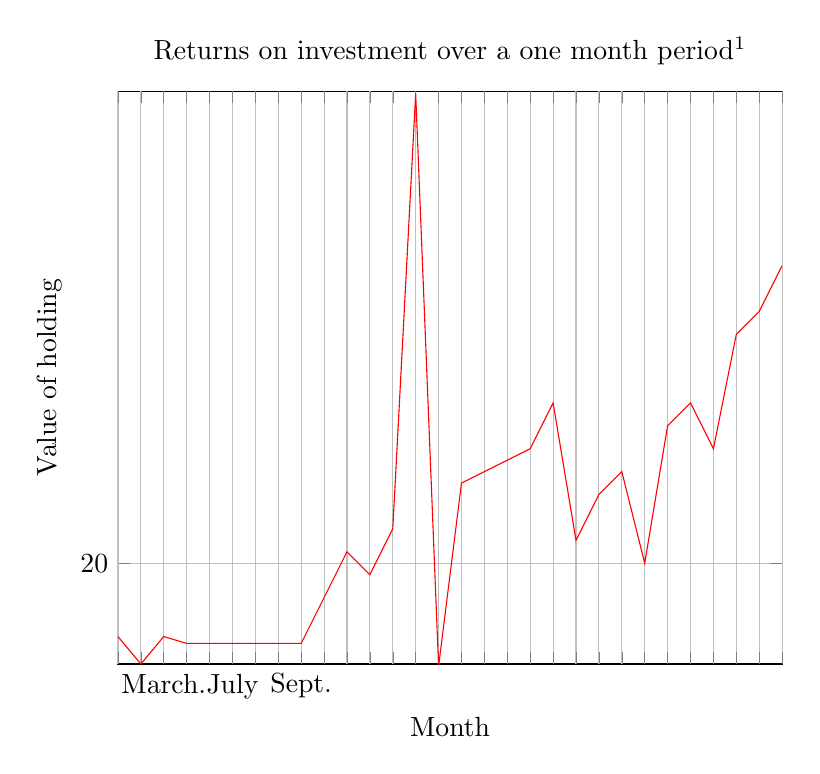
\begin{tikzpicture}
%\draw[step=1cm,gray,very thin] (-2,-2) grid (6,6);
\begin{axis}[
		title={Returns on investment over a one month period\footnote{Values shown}},
       % axis on top,% ----
        grid = both,
        xtick={3,6,9},
        xticklabels={March., July,Sept.},
        extra x ticks={1,2,3,4,5,6,7,8,9,10,11,12,13,14,15,16,17,18,19,20,21,22,23,24,25,26,27,28,29,30},
    		extra x tick style={
        xticklabel={}},
    		ytick={0,10,20,60,80,100,120},
        ylabel= Value of holding,
    		xlabel= Month,
        scale only axis,
        enlargelimits=false,
       % xmin=0,
       % xmax=96,
        ymin=15.6, %min = min observed y value
       % ymax=20.5,
        axis equal=true
        ]
         \addplot [color=red] coordinates { %medium
       (1,16.8) 
       (2,15.6) 
       (3,16.8) 
       (4,16.5)
       (5,16.5)
       (6,16.5)
       (7,16.5)
       (8,16.5)
       (9,16.5)
       (10,18.5)
       (11,20.5)
       (12,19.5)
       (13,21.5)
       (14,40.5)
       (15,15.5)
       (16,23.5)
       (17,24)
       (18,24.5)
       (19,25)
       (20,27)
       (21,21)
       (22,23)
       (23,24)
       (24,20)
       (25,26)
       (26,27)
       (27,25)
       (28,30)
       (29,31)
       (30,33)
    };
\end{axis}
\end{tikzpicture}
\subsection*{One year returns}
 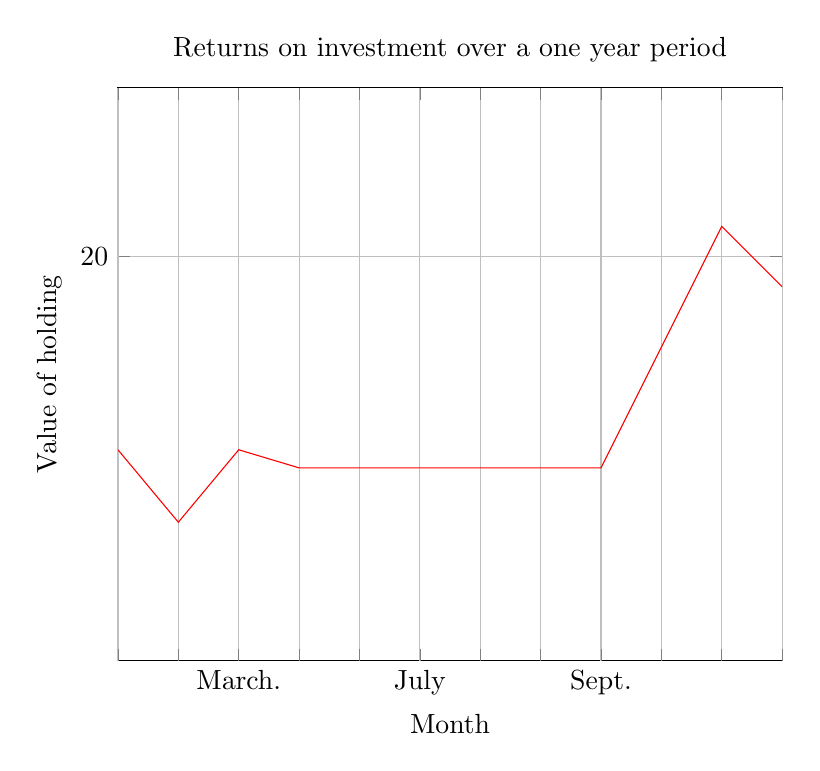
\begin{tikzpicture}
\begin{axis}[
		title={Returns on investment over a one year period},
       % axis on top,% ----
        grid = both,
        xtick={3,6,9},
        xticklabels={March., July,Sept.},
        extra x ticks={1,2,3,4,5,6,7,8,9,10,11,12},
    		extra x tick style={
        xticklabel={}},
    		ytick={0,10,20,60,80,100,120},
        ylabel= Value of holding,
    		xlabel= Month,
        scale only axis,
        enlargelimits=false,
       % xmin=0,
       % xmax=96,
       % ymin=0,
       % ymax=96,
        axis equal=true
        ]
         \addplot [color=red] coordinates { %medium
       (1,16.8) 
       (2,15.6) 
       (3,16.8) 
       (4,16.5)
       (5,16.5)
       (6,16.5)
       (7,16.5)
       (8,16.5)
       (9,16.5)
       (10,18.5)
       (11,20.5)
       (12,19.5)
    };
\end{axis}
\end{tikzpicture} 
\subsubsection{3-year returns}
Plotting from data:

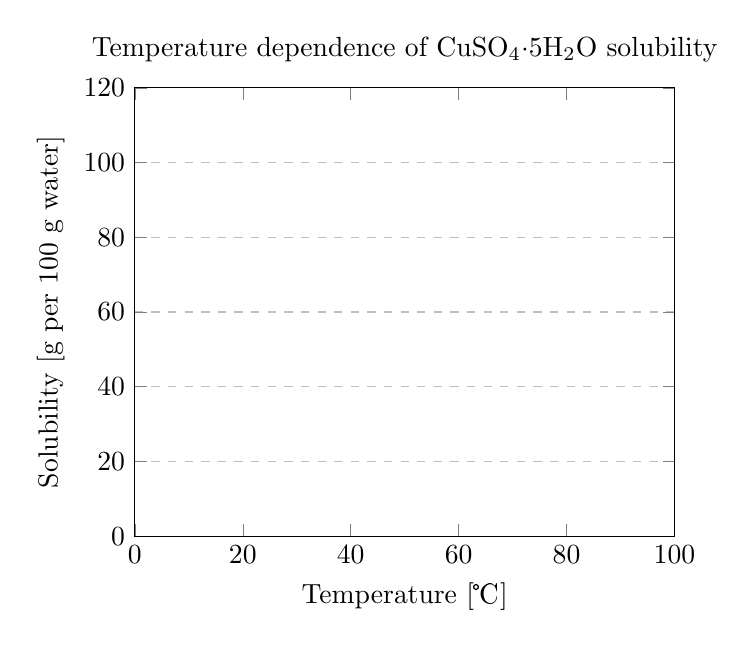
\begin{tikzpicture}
\begin{axis}[
    title={Temperature dependence of CuSO\(_4\cdot\)5H\(_2\)O solubility},
    xlabel={Temperature [\textcelsius]},
    ylabel={Solubility [g per 100 g water]},
    xmin=0, xmax=100,
    ymin=0, ymax=120,
    xtick={0,20,40,60,80,100},
    ytick={0,20,40,60,80,100,120},
    legend pos=north west,
    ymajorgrids=true,
    grid style=dashed,
]


  
    
\end{axis}
\end{tikzpicture}
\subsubsection{5-year returns}
\section*{Distribution of investments}
\subsection*{Distribution by currency and nationality}

\begin{center}


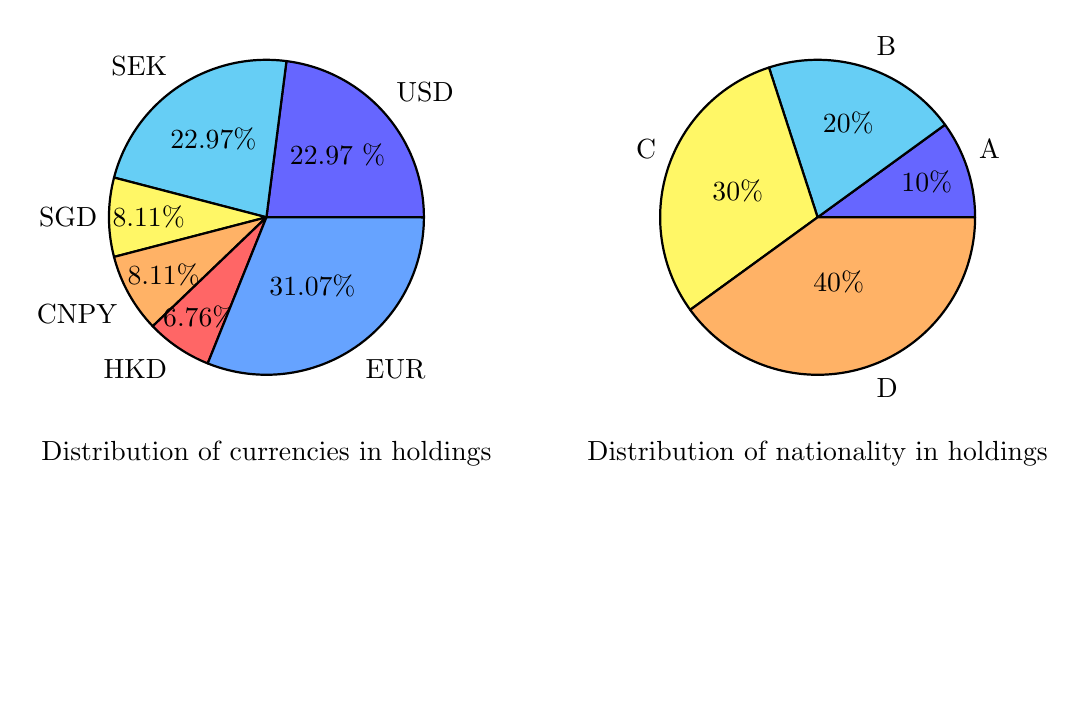
\begin{tikzpicture}[auto=left] 
\node[circle] at (-3,-3) {Distribution of currencies in holdings};
\node[circle] at (4,-3) {Distribution of nationality in holdings};
\pie[
radius=2,
pos={-3,0}
]{
	22.97 / USD,
    22.97/SEK,
    8.11/SGD,
    8.11/CNPY,
    6.76/HKD,
    31.07/EUR
    }
    
\pie[
    radius=2,
    pos={4,0},
]{10/A, 20/B, 30/C, 40/D}


\end{tikzpicture}

\end{center}
\subsection*{Most heavily weighed stocks}
\begin{table}[!h]
\begin{center}


\begin{enumerate}\centering
\item AAPL: 40 \%

\item ASML - 32 \%
\end{enumerate}
\end{center}
\end{table}
\subsection*{Distribution by sector and industry}    

\section*{Information used}
\subsection*{Conversion factors}
\begin{table}[!h]
\begin{center}
\begin{tabular}{||c ||} 
 \hline
 Col1  \\ [0.5ex] 
 \hline\hline
 1  \\ 
 \hline
 2  \\
 \hline
 3  \\
 \hline
 4  \\
 \hline
 5  \\ 
 \hline
\end{tabular}
\caption{Conversion factors for reference currency.}
\end{center}
\end{table}

\begin{table}[!h]
\begin{center}
\begin{tabular}{ |c||c|  }
 \hline
 \multicolumn{2}{|c|}{Country List} \\
 \hline
 \hline
 usd : 1   & EUR : 3\\
 EUR : 3 &   EUR : 3\\
 EUR : 3 & EUR : 3 \\
 EUR : 3   & EUR : 3\\
 EUR : 3 &   EUR : 3 \\
 EUR : 3 & \\
 EUR : 37 &\\
 \hline
\end{tabular}
\caption{Conversion factors for reference currency.}
\end{center}
\end{table}

\end{document}
